% !TEX root = Dokumentation_SysSpec.tex
\subsection{Modelle und Sichten}

\subsubsection{Kontextdiagramm}
Die entwickelte Applikation hat folgende Abhängigkeiten/Umsysteme/Akteuere:
\begin{figure}[H]
	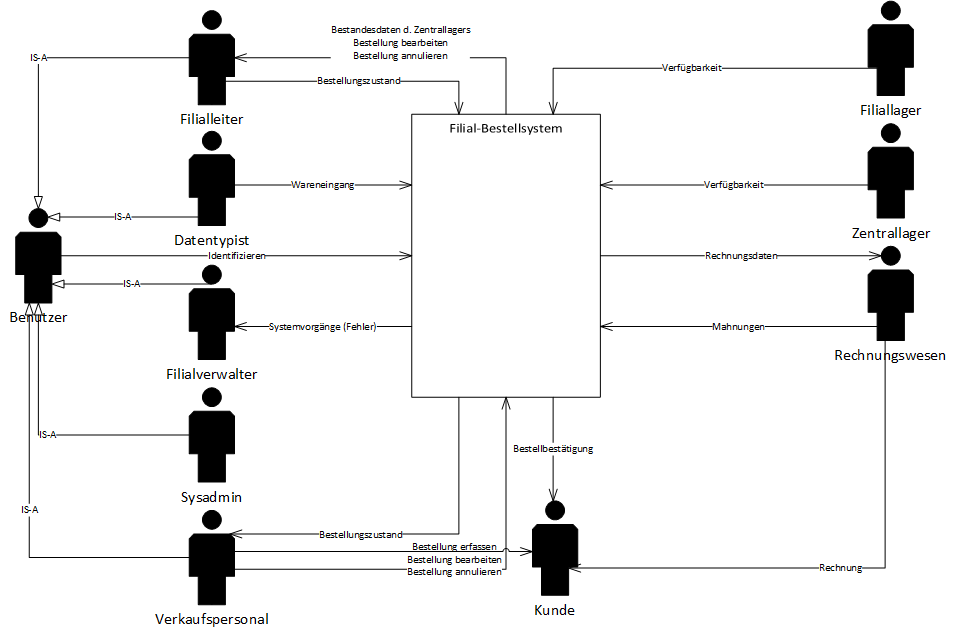
\includegraphics[width=1.0\linewidth]{Images/kontextdiagram}
	\caption{Kontextdiagram}
	\label{fig:kontextdiagram}
\end{figure}

\textbf{Umsysteme}:
\begin{itemize}
\item Zentrallager: Nachbestellungen des lokalen Filiallagers werden an das Zentrallager gesendet.
\item Rechnungswesen: Das Rechnungswesen wird für Bestell-Bestätigungen, Rechnungsversand und Mahnungsprüfungen verwendet.
\item Filiallager: Lagerung der in der Filiale verkauften Artikel. Filiallager und Applikation müssen jederzeit einen übereinstimmenden Datenbestand haben.
\end{itemize}

\textbf{Akteuere}:
\begin{itemize}
\item Benutzer: Bestehend aus Filialverwalter, Filialleiter, Verkaufspersonal und Datentypist, bezeichnet alle Nutzer der Applikation. Die einzelnen Aktionen sind in der Use Case Übersicht ersichtlich
\item Sysadmin: Gemäss Anforderungen kein eigentlicher Benutzer. Für konfigurative Anpassungen könnte ein Zugriff notwendig sein
\item Kunde: Interaktion mit der Applikation wird via Verkaufspersonal abgewickelt.
\end{itemize}

\clearpage
\subsubsection{Layer- \& Tier-Architektur}
Das Filialbestellsystem basiert in der horizontalen Orienterung auf dem 4-Schichten Modell. \\
Der Client-Layer stellt die Interaktionsschicht mit dem Anwender zur Verfügung.\\
Der Remote-Layer dient als Vermittlungsstelle zwischen dem Client- und Business-Layer und führt dadurch zu einer Entkopplung der Anbindung der Clients an den eigentlichen Business-Layer. Weiter ermöglicht dieser Layer in einem weiteren Release, dass der Client-Layer auf mehreren Tiers ohne grössere Aufwendungen betrieben werden könnte.\\
Der Business-Layer übernimmt die Abläufe (auch Workflows) für die zur Verfügung gestellten Bestellungen. Der Business-Layer bindet dabei auch die notwendigen Umsysteme wie Zentrallager, Rechnungswesen an.\\
Der Data-Layer übernimmt die Übersetzung der Business-Aktionen mittels O/R-Mapper auf die Datenbank und ermöglicht so die Persistierung der Daten.\\
Quer durch alle Layer wurden jeweils die entsprechenden funktionalen Anforderungen abgebildet. Jeder der vertikalen Elemente können unter Beachtung der Schnittstellen ausgetauscht / erweitert werden.\\
Dabei wurden folgende vertikalen Elemente umgesetzt:
\begin{itemize}
	\item Order:
	\item SupplyOrder
	\item Article:
	\item Customer:
	\item UserManagement
	\item SessionManagement
\end{itemize}

TODO Übersichsgrafik importieren und erläutern

\subsubsection{Client-Layer}
Der Client-Layer ist in JavaFX implementiert und verwendet das MVC-Architektur-Pattern. Zur Gestaltung der Oberfläche wurde ein 3rd Party Tool eingesetzt, um die graphische Gestaltung zu vereinfachen.
\begin{itemize}
\item Scene Builder by Gluon: Basiert auf der von Oracle entwickelten JavaFX-Distribution, und erstellt ein passendes FXML-Dokument für die Einbindung der graphischen Oberfläche, inklusive Verlinkung und definition der Event-Handler. 
\end{itemize}
\begin{figure}[H]
	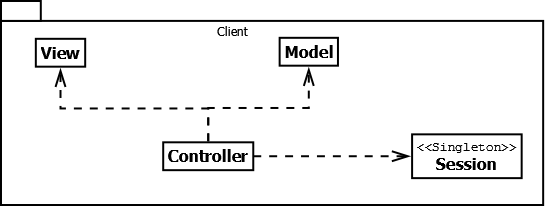
\includegraphics[width=1.0\linewidth]{Images/ClientLayer-Architektur}
	\caption{Architektur des Clientlayer}
	\label{fig:clientlayer-architektur}
\end{figure}

\textbf{View}: Die View ist dafür verantwortlich, dass die angezeigte Oberfläche korrekt geladen ist.

\textbf{Controller}: Die Controller binden die FXML-Dokumente ein. Die Controller registrieren ausgelöste Events und steuern die durchzufürenden Aktionen, wie Datenabfragen vom Business-Layer durch.

\textbf{Model}: Im Model befinden sich die im GUI angezeigten Datenwerte, und sind bereits durch die Verwendung von Property-Klassen als Observable-Objekte abgespeichert.

\textbf{Session}: Die Session enthält die User-Informationen. Die Session-Informationen werden bei Aktionen mitgesendet, um unauthorisierte Aufrufe zu unterbinden.\\\\
\clearpage
Im Layer Client wurden folgende Klassen definiert:
\begin{longtable} {|l|ll|} 
		
		\hline
		\rowcolor{gray!50}\textbf{Package}                                                                                                & \textbf{Klasse}                                                           & \textbf{Aufgabe / Verantwortung}                                                                                                                 \\ \hline \endhead
		ch.hslu.appe.fbs.client                                                                                         & MainApp                                                                   & Einstiegspunkt für GUI-Client                                                                                                                   \\ \hline
		\multirow{12}{*}{\begin{tabular}[c]{@{}l@{}}ch.hslu.appe.fbs.client.\\ controller\end{tabular}}                 & AlertMessage                                                              & \begin{tabular}[c]{@{}l@{}}Erstellt Popup Messages für Warnungen/\\ Fehler\end{tabular}                                                         \\ \cline{2-3} 
		& LandingController                                                         & ??                                                                                                                                              \\ \cline{2-3} 
		& LoginPageController                                                       & \begin{tabular}[c]{@{}l@{}}Controller für LoginPage, behandelt rolen-\\ spezifische Pageselection \& Validierung \\ der Logindaten\end{tabular} \\ \cline{2-3} 
		& MenuBarController                                                         & \begin{tabular}[c]{@{}l@{}}Verantwortlich für MenuBar in Pages \\ (u.a. Exit-Button)\end{tabular}                                               \\ \cline{2-3} 
		& NewOrderController                                                        & \begin{tabular}[c]{@{}l@{}}Controller für die Erstellung einer neuen \\ Bestellung, bindet Remote-Schicht an\end{tabular}                       \\ \cline{2-3} 
		& OrderDetailController                                                     & \begin{tabular}[c]{@{}l@{}}Controller für die Detailansicht einer be-\\ stehenden Bestellung,\\ bindet Remote-Schicht an\end{tabular}           \\ \cline{2-3} 
		& OrderEditController                                                       & \begin{tabular}[c]{@{}l@{}}Controller für die Bearbeitung einer \\ Bestellung, bindet Remote-Schicht an\end{tabular}                            \\ \cline{2-3} 
		& OrderMenuBarController                                                    & Verantwortlich für MenuBar in OrderPages                                                                                                        \\ \cline{2-3} 
		& OrderOverViewController                                                   & \begin{tabular}[c]{@{}l@{}}Controller für die Übersichtstabelle aller \\ bestehenden Bestellungen, \\ bindet Remote-Schicht an\end{tabular}     \\ \cline{2-3} 
		& SupplyMenuBarController                                                   & \begin{tabular}[c]{@{}l@{}}Verantwortlich für MenuBar in \\ SupplyOrderPages\end{tabular}                                                       \\ \cline{2-3} 
		& \begin{tabular}[c]{@{}l@{}}SupplyOrderOver-\\ ViewController\end{tabular} & \begin{tabular}[c]{@{}l@{}}Controller für die Übersichtstabelle aller \\ bestehenden Nachbestellungen, \\ bindet Remote-Schicht an\end{tabular} \\ \cline{2-3} 
		& SupplyPageController                                                      & \begin{tabular}[c]{@{}l@{}}Controller für den Wareneingang von Nach-\\ bestellungen, bindet Remote-Schicht an\end{tabular}                      \\ \hline
		\multirow{6}{*}{\begin{tabular}[c]{@{}l@{}}ch.hslu.appe.fbs.client.\\ controller.userrolestrategy\end{tabular}} & IUserRoleStrategy                                                         & \begin{tabular}[c]{@{}l@{}}Interface für das Handling (Strategy-Pattern)\\ der verschiedenen Userrollen\end{tabular}                            \\ \cline{2-3} 
		& UserRoleContext                                                           & \begin{tabular}[c]{@{}l@{}}Verweisklasse für spezifisches Verhalten \\ anhand Pattern\end{tabular}                                              \\ \cline{2-3} 
		& DatentypistStrategy                                                       & Pagezuweisung anhand Rolle 'Datentypist'                                                                                                        \\ \cline{2-3} 
		& FilialleiterStrategy                                                      & Pagezuweisung anhand Rolle 'Filialleiter'                                                                                                       \\ \cline{2-3} 
		& FilialverwalterStrategy                                                   & Pagezuweisung anhand Rolle 'Filialverwalter'                                                                                                    \\ \cline{2-3} 
		& VerkaufspersonalStrategy                                                  & \begin{tabular}[c]{@{}l@{}}Pagezuweisung anhand \\ Rolle 'Verkaufspersonal'\end{tabular}                                                        \\ \hline
		
		\pagebreak
		\multirow{12}{*}{\begin{tabular}[c]{@{}l@{}}ch.hslu.appe.fbs.client.\\ model\end{tabular}}                      & IUserData                                                                 & Schnittstelle für Benutzerdaten                                                                                                                 \\ \cline{2-3} 
		& UserData                                                                  & \begin{tabular}[c]{@{}l@{}}Repräsentiert die Daten eines Benutzers \\ (Name, Passwort, Rolle)\end{tabular}                                      \\ \cline{2-3} 
		& KeyValuePair                                                              & Unterstützungsklasse für Key/Value Pairs                                                                                                        \\ \cline{2-3} 
		& ArticleData                                                               & \begin{tabular}[c]{@{}l@{}}Repräsentiert die Daten eines Artikels\\  (ID, Name, Preis, Anzahl, etc.)\end{tabular}                               \\ \cline{2-3} 
		& ArticleListData                                                           & \begin{tabular}[c]{@{}l@{}}Repräsentiert die Liste aller Artikel für \\ Übersichten\end{tabular}                                                \\ \cline{2-3} 
		& CustomerData                                                              & \begin{tabular}[c]{@{}l@{}}Repräsentiert die Daten eines Benutzers \\ (ID, Namen)\end{tabular}                                                  \\ \cline{2-3} 
		& CustomerListData                                                          & \begin{tabular}[c]{@{}l@{}}Repräsentiert die Liste aller Kunden \\ für Übersichten\end{tabular}                                                 \\ \cline{2-3} 
		& OrderData                                                                 & \begin{tabular}[c]{@{}l@{}}Repräsentiert die Daten einer Bestellung\\ für die Übersichtsdarstellung\end{tabular}                                \\ \cline{2-3} 
		& OrderDetailData                                                           & \begin{tabular}[c]{@{}l@{}}Repräsentiert die Daten einer Bestellung \\ (bestellte Artikel und Preis)\end{tabular}                               \\ \cline{2-3} 
		& OrderListData                                                             & \begin{tabular}[c]{@{}l@{}}Repräsentiert die Liste aller Bestellungen \\ für Übersichten\end{tabular}                                           \\ \cline{2-3} 
		& SupplyData                                                                & \begin{tabular}[c]{@{}l@{}}Repräsentiert die Daten einer \\ Nachbestellung\end{tabular}                                                         \\ \cline{2-3} 
		& SupplyListData                                                            & \begin{tabular}[c]{@{}l@{}}Repräsentiert die Liste aller \\ Nachbestellungen für Übersichten\end{tabular}                                       \\ \hline
		\multirow{8}{*}{\begin{tabular}[c]{@{}l@{}}ch.hslu.appe.fbs.client.\\ view\end{tabular}}                        & LandingPage                                                               & GUI-Ansicht Landing                                                                                                                             \\ \cline{2-3} 
		& LoginPage                                                                 & GUI-Ansicht Login                                                                                                                               \\ \cline{2-3} 
		& NewOrderPage                                                              & GUI-Ansicht neue Bestellung                                                                                                                     \\ \cline{2-3} 
		& OrderDetailPage                                                           & GUI-Ansicht Bestellungsdetails                                                                                                                  \\ \cline{2-3} 
		& OrderEditPage                                                             & GUI-Ansicht Bestellbearbeitung                                                                                                                  \\ \cline{2-3} 
		& OrderOverviewPage                                                         & GUI-Ansicht Bestellübersicht                                                                                                                    \\ \cline{2-3} 
		& SupplyOrderoverviewPage                                                   & GUI-Ansicht Nachbestellübersicht                                                                                                                \\ \cline{2-3} 
		& SupplyPage                                                                & GUI-Ansicht Wareneingang                                                                                                                        \\ \hline
	\caption{Klassen Layer Client}
	\label{tab:classes-layer-client}
\end{longtable}

\subsubsection{Remote-Layer}
\begin{figure}[H]
	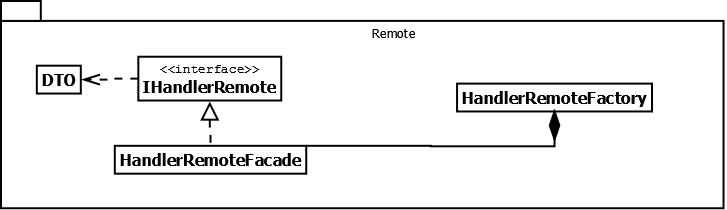
\includegraphics[width=1.0\linewidth]{Images/RemoteLayer-Architektur}
	\caption{Architektur des Remotelayer}
	\label{fig:remotelayer-architektur}
\end{figure}

\clearpage
Im Layer Remote wurden folgende Klassen definiert:
\begin{longtable} {|l|ll|} 	
	\hline
	\rowcolor{gray!50}
		\textbf{Package}                                                                                               & \textbf{Klasse}                          & \textbf{Aufgabe /Verantwortung}                                                                                        \\ \hline
		\endhead
		\multirow{4}{*}{\begin{tabular}[c]{@{}l@{}}ch.hslu.appe.fbs.business.\\ article\end{tabular}}           & IArticleHandlerRemote           & Interface für RemoteFactory                                                                                    \\ \cline{2-3} 
		& ArticleDTO                      & \begin{tabular}[c]{@{}l@{}}Data Transfer Object für einen Artikel \\ zw. Client und Remote\end{tabular}        \\ \cline{2-3} 
		& ArticleHandlerRemoteFactory     & \begin{tabular}[c]{@{}l@{}}Erzeugt ArticleHanderRemoteFacade\\  Objekte\end{tabular}                           \\ \cline{2-3} 
		& ArticleHandlerRemoteFacade      & \begin{tabular}[c]{@{}l@{}}Bindeglied Remote \& Business, \\ übernimmt DTO-zu-Model Konvertierung\end{tabular} \\ \hline
		\multirow{4}{*}{\begin{tabular}[c]{@{}l@{}}ch.hslu.appe.fbs.business.\\ customer\end{tabular}}          & ICustomerHandlerRemote          & Interface für RemoteFactory                                                                                    \\ \cline{2-3} 
		& CustomerDTO                     & \begin{tabular}[c]{@{}l@{}}Data Transfer Object für einen Kunden \\ zw. Client und Remote\end{tabular}         \\ \cline{2-3} 
		& CustomerHandlerRemoteFactory    & \begin{tabular}[c]{@{}l@{}}Erzeugt CustomerHanderRemoteFacade \\ Objekte\end{tabular}                          \\ \cline{2-3} 
		& CustomerHandlerRemoteFacade     & \begin{tabular}[c]{@{}l@{}}Bindeglied Remote \& Business, \\ übernimmt DTO-zu-Model Konvertierung\end{tabular} \\ \hline
		\multirow{4}{*}{\begin{tabular}[c]{@{}l@{}}ch.hslu.appe.fbs.business.\\ order\end{tabular}}             & IOrderHandlerRemote             & Interface für RemoteFactory                                                                                    \\ \cline{2-3} 
		& OrderDTO                        & \begin{tabular}[c]{@{}l@{}}Data Transfer Object für eine Bestellung \\ zw. Client und Remote\end{tabular}      \\ \cline{2-3} 
		& OrderHandlerRemoteFactory       & Erzeugt OrderHanderRemoteFacade Objekte                                                                        \\ \cline{2-3} 
		& OrderHandlerRemoteFacade        & \begin{tabular}[c]{@{}l@{}}Bindeglied Remote \& Business, \\ übernimmt DTO-zu-Model Konvertierung\end{tabular} \\ \hline
		\multirow{4}{*}{\begin{tabular}[c]{@{}l@{}}ch.hslu.appe.fbs.business.\\ supplyorder\end{tabular}}       & ISupplyOrderHandlerRemote       & Interface für RemoteFactory                                                                                    \\ \cline{2-3} 
		& SupplyOrderDTO                  & \begin{tabular}[c]{@{}l@{}}Data Transfer Object für eine Nachbestellung \\ zw. Client und Remote\end{tabular}  \\ \cline{2-3} 
		& SupplyOrderHandlerRemoteFactory & \begin{tabular}[c]{@{}l@{}}Erzeugt SupplyOrderHanderRemoteFacade \\ Objekte\end{tabular}                       \\ \cline{2-3} 
		& SupplyOrderHandlerRemoteFacade  & \begin{tabular}[c]{@{}l@{}}Bindeglied Remote \& Business, \\ übernimmt DTO-zu-Model Konvertierung\end{tabular} \\ \hline
		\multirow{3}{*}{\begin{tabular}[c]{@{}l@{}}ch.hslu.appe.fbs.business.\\ sessionmanagement\end{tabular}} & ISessionHandlerRemote           & Interface für RemoteFactory                                                                                    \\ \cline{2-3} 
		& SessionHandlerRemoteFactory     & Erzeugt SessionHanderRemoteFacade Objekte                                                                      \\ \cline{2-3} 
		& SessionHandlerRemoteFacade      & \begin{tabular}[c]{@{}l@{}}Bindeglied Remote \& Business, \\ übernimmt DTO-zu-Model Konvertierung\end{tabular} \\ \hline 
		
		\pagebreak
		\multirow{4}{*}{\begin{tabular}[c]{@{}l@{}}ch.hslu.appe.fbs.business.\\ usermanagement\end{tabular}}    & IUserHandlerRemote              & Interface für RemoteFactory                                                                                    \\ \cline{2-3} 
		& UserDTO                         & \begin{tabular}[c]{@{}l@{}}Data Transfer Object für einen Benutzer \\ zw. Client und Remote\end{tabular}       \\ \cline{2-3} 
		& UserHandlerRemoteFactory        & Erzeugt UserHanderRemoteFacade Objekte                                                                         \\ \cline{2-3} 
		& UserHandlerRemoteFacade         & \begin{tabular}[c]{@{}l@{}}Bindeglied Remote \& Business, \\ übernimmt DTO-zu-Model Konvertierung\end{tabular} \\ \hline
		\multirow{4}{*}{\begin{tabular}[c]{@{}l@{}}ch.hslu.appe.fbs.business.\\ logmanagement\end{tabular}}     & ILoggerHandlerRemote            & Interface für RemoteFactory                                                                                    \\ \cline{2-3} 
		& LoggerDTO                       & \begin{tabular}[c]{@{}l@{}}Data Transfer Object für einen Logeintrag \\ zw. Client und Remote\end{tabular}     \\ \cline{2-3} 
		& LoggerHandlerRemoteFactory      & Erzeugt LoggerHanderRemoteFacade Objekte                                                                       \\ \cline{2-3} 
		& LoggerHandlerRemoteFacade       & \begin{tabular}[c]{@{}l@{}}Bindeglied Remote \& Business, \\ übernimmt DTO-zu-Model Konvertierung\end{tabular} \\ \hline
	\caption{Klassen Layer Remote}
	\label{tab:classes-layer-remote}
\end{longtable}

\subsubsection{Business-Layer}
Der Business-Layer stellt die administrative und ablaufgesteuerte Schnittstelle zwischen Client und Data-Layer dar. Der Business-Layer hat dabei folgende Aufgaben:\\
- Transaktionhandling bei Bestellungen\\
- 

\begin{figure}[H]
	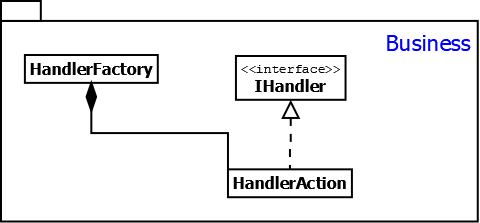
\includegraphics[width=1.0\linewidth]{Images/BusinessLayer-Architektur}
	\caption{Architektur des Businesslayer}
	\label{fig:businesslayer-architektur}
\end{figure}

\clearpage
Im Layer Business wurden folgende Klassen definiert:
\begin{longtable} {|l|ll|} 	
		\hline
		\rowcolor{gray!50}
		\textbf{Package}                                                                                        & \textbf{Klasse}           & \textbf{Aufgabe / Verantwortung}                                                                                                                      \\ \hline
		\endhead
		\multirow{3}{*}{\begin{tabular}[c]{@{}l@{}}ch.hslu.appe.fbs.business.\\ article\end{tabular}}           & IArticleHandler           & Interface HandlerFactory                                                                                                                              \\ \cline{2-3} 
		& ArticleHandlerFactory     & Erzeugt ArticleHandlerAction Objekte                                                                                                                  \\ \cline{2-3} 
		& ArticleHandlerAction      & \begin{tabular}[c]{@{}l@{}}Übernimmt alle Businessaktionen \\ für einen Artikel\end{tabular}                                                          \\ \hline
		\multirow{3}{*}{\begin{tabular}[c]{@{}l@{}}ch.hslu.appe.fbs.business.\\ customer\end{tabular}}          & ICustomerHandler          & Interface HandlerFactory                                                                                                                              \\ \cline{2-3} 
		& CustomerHandlerFactory    & \begin{tabular}[c]{@{}l@{}}Erzeugt CustomerHandlerAction \\ Objekte\end{tabular}                                                                      \\ \cline{2-3} 
		& CustomerHandlerAction     & \begin{tabular}[c]{@{}l@{}}Übernimmt alle Businessaktionen für \\ einen Kunden\end{tabular}                                                           \\ \hline
		\multirow{3}{*}{\begin{tabular}[c]{@{}l@{}}ch.hslu.appe.fbs.business.\\ order\end{tabular}}             & IOrderHandler             & Interface HandlerFactory                                                                                                                              \\ \cline{2-3} 
		& OrderHandlerFactory       & Erzeugt OrderHandlerAction Objekte                                                                                                                    \\ \cline{2-3} 
		& OrderHandlerAction        & \begin{tabular}[c]{@{}l@{}}Übernimmt alle Businessaktionen für \\ eine Bestellung\end{tabular}                                                        \\ \hline
		\multirow{3}{*}{\begin{tabular}[c]{@{}l@{}}ch.hslu.appe.fbs.business.\\ supplyorder\end{tabular}}       & ISupplyOrderHandler       & Interface HandlerFactory                                                                                                                              \\ \cline{2-3} 
		& SupplyOrderHandlerFactory & \begin{tabular}[c]{@{}l@{}}Erzeugt SupplyOrderHandlerAction \\ Objekte\end{tabular}                                                                   \\ \cline{2-3} 
		& SupplyOrderHandlerAction  & \begin{tabular}[c]{@{}l@{}}Übernimmt alle Businessaktionen für \\ einen Nachbestellung \& Wareneingang\end{tabular}                                   \\ \hline
		\multirow{3}{*}{\begin{tabular}[c]{@{}l@{}}ch.hslu.appe.fbs.business.\\ sessionmanagement\end{tabular}} & ISessionHandler           & Interface HandlerFactory                                                                                                                              \\ \cline{2-3} 
		& SessionHandlerFactory     & Erzeugt SessionHandlerAction Objekte                                                                                                                  \\ \cline{2-3} 
		& SessionHandlerAction      & \begin{tabular}[c]{@{}l@{}}Übernimmt alle Businessaktionen \\ für eine Session\end{tabular}                                                           \\ \hline
		\multirow{4}{*}{\begin{tabular}[c]{@{}l@{}}ch.hslu.appe.fbs.business.\\ usermanagement\end{tabular}}    & IUserHandler              & Interface HandlerFactory                                                                                                                              \\ \cline{2-3} 
		& UserHandlerFactory        & Erzeugt UserHandlerAction Objekte                                                                                                                     \\ \cline{2-3} 
		& UserHandlerAction         & \begin{tabular}[c]{@{}l@{}}Übernimmt alle Businessaktionen \\ für einen Benutzer\end{tabular}                                                         \\ \cline{2-3} 
		& UserNotFoundException     & \begin{tabular}[c]{@{}l@{}}Exceptionklasse für nichtgefundene \\ Benutzer\end{tabular}                                                                \\ \hline
		\multirow{3}{*}{\begin{tabular}[c]{@{}l@{}}ch.hslu.appe.fbs.business.\\ logmanagement\end{tabular}}     & ILoggerHandler            & Interface HandlerFactory                                                                                                                              \\ \cline{2-3} 
		& LoggerHandlerFactory      & Erzeugt LoggerHandlerAction Objekte                                                                                                                   \\ \cline{2-3} 
		& LoggerHandlerAction       & \begin{tabular}[c]{@{}l@{}}Übernimmt alle Businessaktionen für \\ einen Loggereintrag\end{tabular}                                                    \\ \hline
		\pagebreak
		\multirow{9}{*}{\begin{tabular}[c]{@{}l@{}}ch.hslu.appe.fbs.business.\\ stubs\end{tabular}}             & ArticleHandlerStub        & \begin{tabular}[c]{@{}l@{}}Stub, welcher mehrere Test-Artikel \\ bereitstellt\end{tabular}                                                            \\ \cline{2-3} 
		& CustomerHandlerStub       & \begin{tabular}[c]{@{}l@{}}Stub, welcher mehrere Test-Kunden \\ bereitstellt\end{tabular}                                                             \\ \cline{2-3} 
		& FinanceStub               & \begin{tabular}[c]{@{}l@{}}Repräsentation des Rechnungswesens \\ mit der Möglichkeit für Rechnungsstellung \\ und Überprüfung Mahnstatus\end{tabular} \\ \cline{2-3} 
		& OrderHandlerStub          & \begin{tabular}[c]{@{}l@{}}Stub, welcher mehrere Test-Bestellungen \\ inkl. Bezug auf Kunde \& Artikel anbietet\end{tabular}                          \\ \cline{2-3} 
		& PerimeterStub             & \begin{tabular}[c]{@{}l@{}}Stub für den Ausdruck von Bestell-\\ informationen\end{tabular}                                                            \\ \cline{2-3} 
		& SessionHandlerStub        & \begin{tabular}[c]{@{}l@{}}Stub übernimmt die Zuweisung der \\ Berechtigung zu der Userrolle (Context)\end{tabular}                                   \\ \cline{2-3} 
		& StockStub                 & Repräsentation des Zentrallagers                                                                                                                      \\ \cline{2-3} 
		& SupplyOrderHandlerStub    & \begin{tabular}[c]{@{}l@{}}Stub, welcher mehrere Test-Nach-\\ bestellungen bereitstellt\end{tabular}                                                  \\ \cline{2-3} 
		& UserHandlerStub           & \begin{tabular}[c]{@{}l@{}}Stub, welcher mehrere Test-User \\ bereitstellt\end{tabular}                                                               \\ \hline
	\caption{Klassen Layer Business}
	\label{tab:classes-layer-business}
\end{longtable}

\subsubsection{Data-Layer}
\begin{figure}[H]
	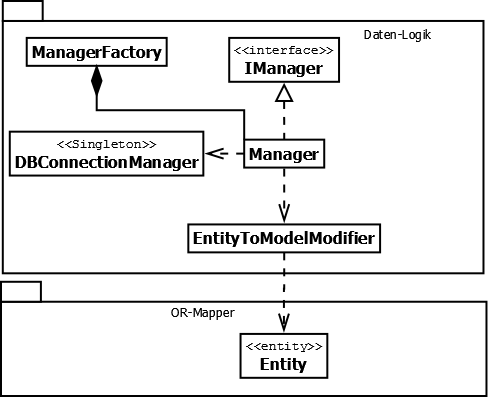
\includegraphics[width=1.0\linewidth]{Images/DataLayer-Architektur}
	\caption{Architektur des Datalayer}
	\label{fig:datalayer-architektur}
\end{figure}

\clearpage
Im Layer Data wurden folgende Klassen definiert:
\begin{longtable} {|l|ll|} 	
		\hline
		\rowcolor{gray!50}
		\textbf{Package}                                                                              & \textbf{Klasse}                       & \textbf{Aufgabe / Verantwortung}                                                         \\ \hline
		\endhead
		ch.hslu.appe.fbs.data                                                                         & DBConnectionManager                   & \begin{tabular}[c]{@{}l@{}}Stellt Verbindung zu \\ mySQL DB her\end{tabular}             \\ \hline
		\multirow{4}{*}{\begin{tabular}[c]{@{}l@{}}ch.hslu.appe.fbs.data.\\ article\end{tabular}}     & IArticleManager                       & \begin{tabular}[c]{@{}l@{}}Interface für Artikel zu \\ Business\end{tabular}             \\ \cline{2-3} 
		& ArticleManager                        & \begin{tabular}[c]{@{}l@{}}Handling von Artikel \\ gegenüber DB\end{tabular}             \\ \cline{2-3} 
		& ArticleManagerFactory                 & \begin{tabular}[c]{@{}l@{}}Erzeugt ArticleManager \\ Objekte\end{tabular}                \\ \cline{2-3} 
		& ArticleEntityToArticleModelModifier   & \begin{tabular}[c]{@{}l@{}}Konvertierungsklasse von \\ DB-Entität zu Model\end{tabular}  \\ \hline
		\multirow{4}{*}{\begin{tabular}[c]{@{}l@{}}ch.hslu.appe.fbs.data.\\ customer\end{tabular}}    & ICustomerManager                      & \begin{tabular}[c]{@{}l@{}}Interface für Kunden zu \\ Business\end{tabular}              \\ \cline{2-3} 
		& CustomerManager                       & \begin{tabular}[c]{@{}l@{}}Handling von Kunden \\ gegenüber DB\end{tabular}              \\ \cline{2-3} 
		& CustomerManagerFactory                & \begin{tabular}[c]{@{}l@{}}Erzeugt CustomerManager \\ Objekte\end{tabular}               \\ \cline{2-3} 
		& CustomerEntityToCustomerModelModifier & \begin{tabular}[c]{@{}l@{}}Konvertierungsklasse von \\ DB-Entität zu Model\end{tabular}  \\ \hline
		\multirow{6}{*}{\begin{tabular}[c]{@{}l@{}}ch.hslu.appe.fbs.data.\\ order\end{tabular}}       & IOrderManager                         & \begin{tabular}[c]{@{}l@{}}Interface für Bestellungen zu \\ Business\end{tabular}        \\ \cline{2-3} 
		& OrderManager                          & \begin{tabular}[c]{@{}l@{}}Handling von Bestellungen \\ gegenüber DB\end{tabular}        \\ \cline{2-3} 
		& OrderManagerFactory                   & \begin{tabular}[c]{@{}l@{}}Erzeugt OrderManager \\ Objekte\end{tabular}                  \\ \cline{2-3} 
		& OrderEntityToOrderModelModifier       & \begin{tabular}[c]{@{}l@{}}Konvertierungsklasse von \\ DB-Entität zu Model\end{tabular}  \\ \cline{2-3} 
		& OrderModelToOrderEntityModifier       & \begin{tabular}[c]{@{}l@{}}Konvertierungsklasse von \\ Model zu DB-Entität\end{tabular}  \\ \cline{2-3} 
		& OrderStatesManager                    & \begin{tabular}[c]{@{}l@{}}Übernimmt Handling von \\ Bestellzuständen\end{tabular}       \\ \hline
		\multirow{3}{*}{\begin{tabular}[c]{@{}l@{}}ch.hslu.appe.fbs.data.\\ stock\end{tabular}}       & IStockManager                         & \begin{tabular}[c]{@{}l@{}}Interface für Lagerartikel zu \\ Business\end{tabular}        \\ \cline{2-3} 
		& StockManager                          & \begin{tabular}[c]{@{}l@{}}Handling von Lagerartikel \\ gegenüber DB\end{tabular}        \\ \cline{2-3} 
		& StockManagerFactory                   & Erzeugt StockManager Objekte                                                             \\ \hline
		\pagebreak
		
		\multirow{3}{*}{\begin{tabular}[c]{@{}l@{}}ch.hslu.appe.fbs.data.\\ supplyorder\end{tabular}} & ISupplyOrderManager                   & \begin{tabular}[c]{@{}l@{}}Interface für Nachbestellungen zu \\ Business\end{tabular}    \\ \cline{2-3} 
		& SupplyOrderManager                    & \begin{tabular}[c]{@{}l@{}}Handling von Nachbestellungen \\ gegenüber DB\end{tabular}    \\ \cline{2-3} 
		& SupplyOrderManagerFactory             & \begin{tabular}[c]{@{}l@{}}Erzeugt SupplyOrderManager \\ Objekte\end{tabular}            \\ \hline
		\multirow{3}{*}{\begin{tabular}[c]{@{}l@{}}ch.hslu.appe.fbs.data.\\ user\end{tabular}}        & IUserManager                          & \begin{tabular}[c]{@{}l@{}}Interface für Benutzer zu \\ Business\end{tabular}            \\ \cline{2-3} 
		& UserManager                           & \begin{tabular}[c]{@{}l@{}}Handling von Benutzern \\ gegenüber DB\end{tabular}           \\ \cline{2-3} 
		& UserManagerFactory                    & Erzeugt UserManager Objekte                                                              \\ \hline
		\multirow{2}{*}{\begin{tabular}[c]{@{}l@{}}ch.hslu.appe.fbs.data.\\ exception\end{tabular}}   & OrderNotFoundInDatabaseException      & \begin{tabular}[c]{@{}l@{}}Exceptionklasse für Bestellung \\ nicht gefunden\end{tabular} \\ \cline{2-3} 
		& UserNotFoundInDatabaseException       & \begin{tabular}[c]{@{}l@{}}Exceptionklasse für Benutzer \\ nicht gefunden\end{tabular}   \\ \hline
		\multirow{13}{*}{\begin{tabular}[c]{@{}l@{}}ch.hslu.appe.fbs.\\ db\_entities\end{tabular}}    & Address                               & DB-Entität Address                                                                       \\ \cline{2-3} 
		& Article                               & DB-Entität Article                                                                       \\ \cline{2-3} 
		& City                                  & DB-Entität City                                                                          \\ \cline{2-3} 
		& Customer                              & DB-Entität Customer                                                                      \\ \cline{2-3} 
		& Order                                 & DB-Entität Order                                                                         \\ \cline{2-3} 
		& OrderArticle                          & DB-Entität Order-Article                                                                 \\ \cline{2-3} 
		& Orderstatus                           & DB-Entität Orderstatus                                                                   \\ \cline{2-3} 
		& Stock                                 & DB-Entität Stock                                                                         \\ \cline{2-3} 
		& Street                                & DB-Entität Street                                                                        \\ \cline{2-3} 
		& Supplyorder                           & DB-Entität SupplyOrder                                                                   \\ \cline{2-3} 
		& SupplyorderArticle                    & \begin{tabular}[c]{@{}l@{}}DB-Entität SupplyOrder\\ -Article\end{tabular}                \\ \cline{2-3} 
		& User                                  & DB-Entität User                                                                          \\ \cline{2-3} 
		& UserRole                              & DB-Entität UserRole                                                                      \\ \hline
	\caption{Klasse Layer Data}
	\label{tab:classes-layer-data}
\end{longtable}

\subsubsection{UML-Klassendiagramme}
todo


\subsubsection{Sequenzdiagramme}
todo


\subsection{Entwurfsentscheid}
Im Rahmen der Architekturausarbeitung wurden folgende Entwurfsentscheide gefällt:
\begin{itemize}
	\item Für Testzwecke und statische Datenstrukturen werden teilweise Stubs eingesetzt. Beispielsweise sind die Zuweisung Benutzerrollen zu deren Berechtigungen bis Release 1.0 als Stub abgebildet.
	\item Der Business-Layer und Data-Layer (ohne Datenbank, nur OR-Mapper) befinden sich auf dem gleichen Tier. Bis Release 1.0 werden, aus zeitlichen Gründen, keine Bestrebungen zur Aufteilung dieser Layers auf verschiedene Tiers vorgenommen
	\item Die Tier-übergreifende Kommunikation zwischen Tier Client und Business wird mittels RMI (Remote Method Invocation) umgesetzt. Eine alternative Anbindung bspw. mit REST (Representational state transfer) wird nach Release 1.0 in Betracht gezogen.
	\item Als GUI-Komponente auf Layer Client wird JavaFX verwendet.
	\item Als Datenbank wird eine MySQL-Instanz aus dem EnterpriseLab der HSLU verwendet.
	\item Bis Release 1.0 müssen neue Kunden \& Artikel in der Datenbank manuell erfasst / abgebildet werden. Diese werden idealerweise mit einer zentralen Benutzerverwaultung (Rechnungswesen, Zentrallager) in folgenden Releases zusammengeführt.
	\item Die Rechnungsdaten und Mahnungen werden aufgrund in einem Stub generiert. Die Anbindung eines beliebigen, externen Rechnungswesen ist dadurch in folgenden Releases schneller zu bewältigen.
\end{itemize}

TODO
- Dateien einbinden (DB) -> Transaktionsmanagement


\subsection{Datenmodell}
Der Aufbau der Datenbank ist in folgender Abbildung dargestellt.
\begin{figure}[H]
	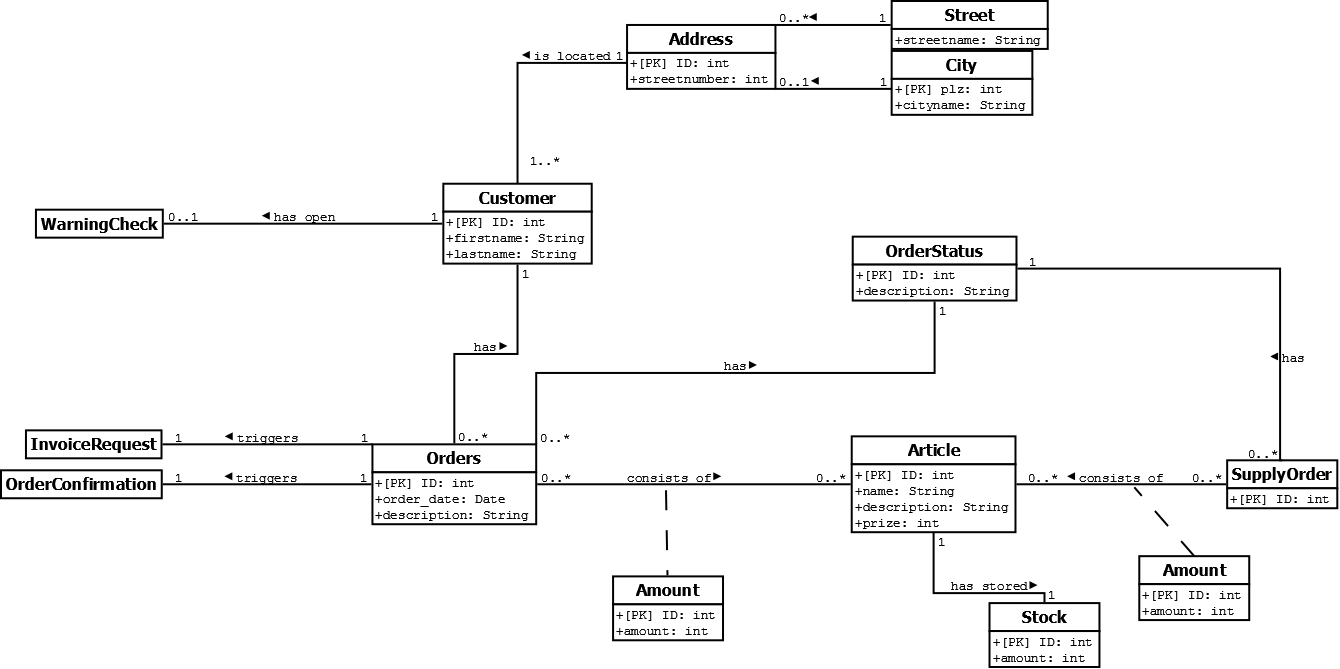
\includegraphics[width=1.0\linewidth]{Images/datamodel}
	\caption{Datenmodel}
	\label{fig:datamodel}
\end{figure}
Die Datenbank ist funktional aufgebaut und befolgt die ersten 3 Normalformen. Die Anbindung von Umsystemen sind im Datenmodell bereits abgebildet, sind jedoch nicht in der Datenbank vorhanden. Die abgebildeten Umsysteme sind WarningCheck, InvoiceRequest und OrderConfirmation.
